% Marco Teorico.
\chapter{Marco te'orico} \label{chap:ssimilar}

AQU\'I VA EL CONTENIDO DEL MARCO TE\'ORICO.
%Puedes quitar esto(es opcional)
\vspace{5 mm}

Los conceptos claves acerca de lo que es un sistema ERP, SAP, ABAP, Ascendant SAP son los que se presentan en este capítulo.

La secci'on \ref{sect:erp} presenta las nociones b'asicas acerca de en qu'e consiste un Sistema de Informaci'on ERP. La secci'on 
\ref{sect:sap} describe un poco lo que es SAP: sus caracter'isticas principales, una  breve historia. Por otro lado, la secci'on \ref{sect:abap} explica en que consiste el lenguaje de programaci'on ABAP, sus principales caracter'isticas. La 'ultima secci'on define la metodolog'ia \textbf{Ascendant SAP (ASAP)}, a ser utilizada a lo largo de este proyecto.

\section{Sistemas de Informaci'on ERP} \label{sect:erp}

Para entender en qu'e consisten los Sistemas de Informaci'on ERP, para ello habr'a que definir dos conceptos fundamentales: Sistema de Informaci'on, y m'as a'un, Sistemas ERP. 

\subsection{Definiciones} \label{subsect:defprop}

\begin{definicion} \label{def:sisinfo}

\end{definicion}

\begin{definicion} \label{def:siserp}
Un ERP (Sistema de Planificación de Recursos Empresariales, 'o como se le conoce en Ingl'es: \textbf{Enterprise Resource Planning}), es un sistema que tiene la capacidad de la automatizaci'on e integraci'on de todos los m'odulos de un 'area de negocio. En otras palabras, es capaz de manejar todas las 'areas relacionadas con una empresa de forma automatizada e integrada. 

Una caracter'istica fundamental de este tipo de sistemas es que est'a basado en m'odulos. Como consecuencia de ello, el mismo est'a compuesto por un conjunto de softwares o m'odulos. 

Para poder tener acceso a los datos que est'an relacionados con cada m'odulo es necesario tener una Base de Datos centralizada, la cual almacena dicha informaci'on. 
\end{definicion}

\section{SAP} \label{sect:sap}

En esta secci'on se ofrece un panorama general acerca de SAP, qu'e es, cu'ales son sus caracter'isticas principales y cu'ales son los m'odulos que lo integra.

\subsection{Definici'on} \label{subsect:defprop}
\textbf{SAP AG} es una empresa de la rama de la Computaci'on que fue fundada por 4 ingenieros pertenecientes a IBM (\textbf{International Business Machines}), en la ciudad de Walldorf, Alemania, en el a~no de 1972. Por su origen alem'an, las siglas SAP son un acr'onimo de: \textit{Systeme, Anwendungen Produkte in der Datenverarbeitung}, que traducido al castellano significa: \textbf{Sistemas, Aplicaciones y Productos en Procesamiento de Datos}. 

El Software principal desarrollado por esta empresa es \textbf{\textit{SAP R/3}} y el cual se encuentra disponible en 28 idiomas. 'Este software es personalizable, utiliza la arquitectura cliente-servidor, es decir, que el cliente envia solicitudes al servidor y 'este a su vez envia una respuesta al cliente. 'Este software fue hecho en el lenguaje de programaci'on \textbf{ABAP/4}. 

\subsection{Caracter'isticas de SAP R/3}
De acuerdo al autor de \cite{SAP01}, las caracter'isticas del software \textbf{SAP R/3} se pueden dividir en diferentes categor'ias, las cuales se mencionan a continuaci'on:

\subsubsection{Caracter'isticas Generales}
\begin{itemize}
\item Es un software altamente integrado y multifuncional, lo que trae como consecuencia que exista una estrecha relaci'on entre las funciones del mismo.
\item Es una aplicaci'on que trabaja en tiempo real. En otras palabras, las actualizaciones de los datos son efectuadas a trav'es de una conexi'on, y en ese mismo instante.
\end{itemize}
\subsubsection{Caracter'isticas de Negocio}
\begin{itemize}
\item Este software contiene todas las funcionalidades necesarias para poder llevar a cabo el manejo de un negocio entero. 'Este incorpora una aplicaci'on llamada \textit{Best Industry Practices}, que traducido al espa\~nol quiere decir: \textit{Mejores Practicas de la Industria}, y 'este 'ultimo es adecuado para una amplia gama de industrias y organizaciones.
\item Este programa es capaz de soportar todos los procesos de negocio de la empresa.
\end{itemize}

\subsubsection{Caracter'isticas de Flexibilidad}
\begin{itemize}
\item Este software es altamente configurable. En otras palabras, se puede adaptar a las necesidades de la empresa que lo utilice y a sus requerimientos. Para ello, se pueden realizar cambios que, dependiendo del n'umero de factores que participen, 'estos tendr'an su grado de complejidad.
\item Es capaz de dar apoyo a empresas que poseen subsidiarias en distintas partes del mundo.
\item Este software es muy utilizado a nivel mundial, dado que est'a disponible en 28 idiomas, y a que posee la capacidad de adaptarse a la moneda, leyes y regulaciones, impuestos para un cierto pa'is, etc.
\end{itemize}

\subsubsection{Caracter'isticas T'ecnicas}
\begin{itemize}
\item Este software tiene la capacidad de ser portable, dado que es multiplataforma, es decir, soporta cualquier sistema operativo, manejador de Base de Datos, etc.
\item Posee un n'umero m'inimo de redundancia, lo que favorece a la consistencia de los datos almacenados. Adicionalmente, posee un manejador de alta seguridad de los datos, y puede manejar etructuras de datos complejas.
\end{itemize}

\subsubsection{Otras Caracter'isticas}
\begin{itemize}
\item Tiene la capacidad de manejar la misma informaci'on en cada m'odulo.
\item Posee una 'unica manera de ingreso al sistema. 'Este es a trav'es del \textit{SAP GUI}.
\item Tiene la capacidad de ser escalable, es decir, que est'a preparado para manejar el continuo crecimiento del trabajo sin disminuir la calidad.
\item Tiene una interfaz gr'afica amigable.
\end{itemize}

\subsection{Adaptaci'on del Software a las Empresas}
Para poder realizar la adaptaci'on de SAP a las necesidades de una empresa en particular, est'an un conjunto de herramientas y utilidades destinado a ello. Para esto, se requiere de un conjunto de consultores, un equipo de proyecto y personal de Tecnolog'ia de la Informaci'on (IT), quienes ser'an los encargados de efectuar dicha adaptaci'on. 

Este proceso se puede realizar a trav'es de dos m'etodos, los cuales se listan a continuaci'on:

\begin{itemize}
\item \textbf{Cambios en la Configuraci'on:} Aqu'i son modificadas las tablas relacionadas con los distintos m'odulos para poder realizar la adaptaci'on.
\item \textbf{Programaci'on en el Lenguaje ABAP/4:} Esto implica modificar programas ya existentes en \textbf{SAP R/3} o crear programas nuevos.
\end{itemize}

\subsection{M'odulos de SAP R/3}
Debido a que SAP es un ERP, luego, SAP est'a dividido en diferentes m'odulos, con el fin de poder abarcar cada 'area de una empresa. Estos m'odulos son los que se listan a continuaci'on:

\begin{enumerate}
\item Asset Management (Manejo de Aplicaciones - AM)
\item Financials (Finanzas - FI)
\item Controlling (Control - CO)
\item Human Resources (Recursos Humanos - HR)
\item Plant Maintenance (Mantenimiento de Planta - PM)
\item Production Planning (Planificaci'on de la Producci'on - PP)
\item Project System (Sistema de Proyectos - PS)
\item Quality Management (Manejo de Calidad -QM)
\item Sales and Distribution (Ventas y Distribuci'on - SD)
\item Materials Management (Manejo de Materiales - MM)
\item Services Management (Manejo de Servicios - SM)
\item Industry Specific Solutions (Soluciones Espec'ificas para la Industria - IS)
\item Business Workflow (Flujo de trabajo del Negocio - WF)
\item Basis (Incluye el lenguaje de programaci'on \textbf{ABAP 4} - BC).

\end{enumerate}

\section{M'odulo de Ventas y Distribuci'on (SD)} \label{sect:sd}

El \textbf{M'odulo de Ventas y Distribuci'on} (Sales and Distribution como es conocido en ingl'es) es un sub-sistema perteneciente a SAP, el cual se encarga de prestar apoyo a las distintas empresas en el 'area de las Ventas y distribuci'on de productos y/o servicios. 

Este m'odulo ayuda a las compa\~n'ias a establecer un precio para sus productos, chequear 'ordenes de ventas que se mantienen abiertas, a tomar previsiones para necesidades futuras, etc. Adicionalmente, ayuda a dar mayor control a las actividades relacionadas con el 'area de ventas: desde el momento en que ocurre un pedido de alg'un(algunos) producto(s) y/o servicio(s) hasta su posterior entrega.

\subsection{Herramientas Principales}
\subsubsection{Manejo de Precios e Impuestos}
A trav'es de esta herramienta, el m'odulo puede evaluar los precios que son colocados a los productos o servicios de acuerdo a unas condiciones establecidas previamente. 
\subsubsection{Chequeo de Disponibilidad}
Con esta herramienta, el m'odulo puede evaluar la disponibilidad de un producto para un almac'en especificado.
\subsubsection{Manejo de Cr'edito}
Con esta herramienta es posible establecer l'imites de cr'edito para un cliente durante el proceso de ventas en el cual se encuentra envuelto.
\subsubsection{Facturaci'on}
Una vez que una Orden de Ventas es creada, se utiliza esta herramienta para crear la(s) factura(s) asociadas.
\subsubsection{Determinaci'on del Material}
Con esta herramienta es posible determinar un material específico de acuerdo a unas condiciones especificadas.
\subsubsection{Determinaci'on de Cuentas}
Ayuda a obtener ciertos detalles de los clientes bas'andose en unas condiciones espec'ificas.
\subsubsection{Procesamiento de Textos}
Con esta herramienta se hace posible el manejo de textos entre los distintos documentos que se obtienen del proceso de ventas.


\subsection{Clasificaci'on de los Datos en el M'odulo SD}
De acuerdo al autor de \cite{SD01}, la data almacenada dentro del M'odulo se puede clasificar como se muestra en la siguiente figura:
\begin{figure}[htb]
\centering
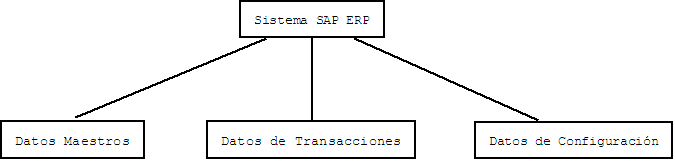
\includegraphics[scale=0.45,type=png,ext=.png,read=.png]{figures/Clasificacion1}
\caption{Clasificaci'on de los datos en el M'odulo SD}
\label{fig:datasd}
\end{figure}
Ahora se proceder'a a explicar la clasificaci'on antes mencionada.
\subsubsection{Datos Maestros}
Los Datos Maestros dentro del M'odulo SD est'an compuestos por:
\begin{itemize}
\item Datos de Compa\~n'ias
\item Datos Maestros de Clientes
\end{itemize}
Cada una de estas entidades contienen a su vez atributos, jerarqu'ias y tablas.

\subsection{Proceso de Ventas utilizando el M'odulo SD}

\subsection{Relaci'on existente entre el M'odulo SD y otros M'odulos}
E'ste m'odulo esta fuertemente integrado con otros m'odulos de SAP, como por ejemplo: MM, WM, QM. 
En el momento en que un cliente realiza un pedido de alg'un producto, posteriormente se chequea la disponibilidad del mismo en alg'un almac'en; esto es posible gracias al m'odulo MM. 
Por otro lado, el m'odulo QM es el encargado de manejar la calidad y brindar soporte a un servicio prestado al cliente, ambos representados por un documento de ventas en SD. 

\section{Lenguaje de Programaci'on ABAP/4}
ABAP (Advanced Business Application Programming - Programaccion de Aplicaciones de Negocio Avanzado) es un lenguaje de programaci'on que fue dise\~nado en la d'ecada de los 80. Su uso principal es la de generar reportes con los cuales se les permite a las empresas construir sus propias aplicaciones para el manejo de las distintas 'areas que lo componen (manejo de materiales, manejo del 'area financiera, manejo de las ventas, etc).
Este es uno de los primeros lenguajes de programación que incluye dentro de su definición el concepto de Bases de Datos L'ogicas. 
Dentro de las caracter'isticas que posee el lenguaje, se pueden mencionar las siguientes:
\begin{itemize}
\item Es un lenguaje basado en la programaci'on estructurada. En otras palabras, contiene estructuras de control.
\item Es un lenguaje interpretado, aunque existen versiones compiladas del mismo.
\item Es muy utilizado para obtener dos tipos de programas: los que son usados para obtener por ejemplo un listado (modo reporte), y aquellos que son usados como transacciones (modo di'alogo).
\item Es un lenguaje orientado a eventos, es decir, que puede ser controlado desde el exterior a trav'es de sentencias de eventos.
\item Est'a integrado totalmente con el sistema \textbf{SAP R/3}.
\item La salida de sus programas es multilingual. 
\end{itemize}
\section{Metodolog'ia Ascendant SAP}
La metodolog'ia \texttt{Ascendant SAP (ASAP)} abarca un proceso estructurado en distintas fases para poder llevar a cabo la gesti'on de un proyecto a ser desarrollado  en SAP, que pueda ser adaptado a las necesidades y requerimientos de la empresa, de manera r'apida y flexible. Esta metodolog'ia fue creada en 1996, y es capaz de dar apoyo a la gerencia de un proyecto, de un equipo de personas, consultores del proceso de negocio, consultores externos y a las distintas 'areas t'ecnicas.
Las principales caracter'isticas de ASAP son las que se listan a continuaci'on:
\begin{itemize}
\item Es capaz de optimizar el tiempo de desarrollo, la calidad del producto final y los recursos empleados.
\item Es capaz de explotar las mejores pr'acticas del negocio.
\item Es capaz de ofrecer un mapa del proyecto orientado a procesos (Hoja de Ruta ASAP) (Ver Anexo).
\item Determina y hace un recorte de los costos de implementaci'on y del tiempo estimado.
\item Ofrece procesos, herramientas, entrenamiento y servicio.
\item Ofrece ayuda detallada a trav'es de cada fase.
\item Es capaz de proveer listas de control, cuestionarios y gu'ias t'ecnicas.
\item Ofrece mejoras de forma continua.
\end{itemize}
Es importante resaltar que esta tecnolog'ia no es utilizada en todos los desarrollos con SAP, ya que la misma se recomienda para aquellas empresas que no tienen una extensa modificaci'on en sus requerimientos, o para aquellas empresas que requieren del uso de la re-ingenier'ia.
Esta metodolog'ia est'a dividida en 4 fases, las cu'ales se listan a continuaci'on:
\subsection{Fase 1: Preparaci'on del Proyecto}
\subsection{Fase 2: Business Blueprint}
\subsection{Fase 3: Realizaci'on}
\subsection{Fase 4: Preparaci'on Final}

